% =====================================================================
%  AI ACADEMY — IEEE CONFERENCE-STYLE REPORT
%  Deep Learning Final Project
%
%  IMPORTANT:
%  Compile with XeLaTeX in Overleaf:
%  Menu -> Settings -> Compiler -> XeLaTeX
% =====================================================================
\documentclass[conference]{IEEEtran}
\usepackage{cite}
\usepackage{amsmath,amssymb,amsfonts}
\usepackage{graphicx}
\usepackage{booktabs}
\usepackage{url}
\usepackage{fontspec}
\usepackage{microtype}
\setmainfont{Liberation Serif}
\newfontfamily\azfont{DejaVu Serif}
\begin{document}
\title{Real-Time Financial Fraud Detection with Learned Hybrid Gating and Uncertainty-Aware Triage}
\author{
\IEEEauthorblockN{
{\azfont Əskərov, Nadir},
{\azfont Fətəliyev, Akşin},
{\azfont Hüseynov, Habil},
{\azfont Nəzərov, Səbuhi}
}
\IEEEauthorblockA{
AI Academy, National Artificial Intelligence Center, Azerbaijan\\
Email: habil.huseynov25@aiacademy.edu.az
}
}
\maketitle
\begin{abstract}
Financial fraud detection is challenging because fraudulent transactions are rare,
behavior evolves over time, and operational systems must distinguish confident
predictions from cases requiring human investigation. We present an end-to-end
fraud detection and uncertainty-triage system that combines supervised and
unsupervised deep learning. An FT-CAT Transformer produces supervised fraud
probabilities from current and historical transaction information, while a
denoising autoencoder provides an independent reconstruction-based anomaly
signal. A learned gating network dynamically combines these signals with
transaction-history activity and amount-intensity features. Split conformal
prediction converts the fused fraud score into operational prediction sets for
automatic approval, automatic blocking, or human review. On the chronological
held-out test set, the FT-CAT model achieved a PR-AUC of 0.3259 and ROC-AUC of
0.8172. At a target miscoverage level of 0.01, the conformal system achieved
98.99\% empirical marginal coverage with a 95\% bootstrap confidence interval of
98.92--99.06\%, while assigning 23.19\% of transactions to human review.
CPU benchmarking measured a median batch-1 neural inference latency of 6.56 ms
and peak tested throughput of approximately 2,746 transactions per second at
batch size 128. The system additionally provides SHAP-based anomaly explanations,
a Streamlit analyst dashboard, FastAPI serving, and EXIR and ONNX model
serialization. Repository:
\url{https://github.com/sa6uhi/DL-final-project}.
\end{abstract}
\begin{IEEEkeywords}
financial fraud detection, deep learning, transformer, anomaly detection,
conformal prediction, uncertainty quantification
\end{IEEEkeywords}
\section{Introduction}
\label{sec:intro}
Financial transaction systems must identify fraudulent behavior under severe
class imbalance while operating under strict latency and reliability
requirements. A useful fraud-detection product must therefore do more than
produce a binary prediction. It should combine complementary evidence, expose
uncertain cases to analysts, provide interpretable information about suspicious
transactions, and remain deployable on modest hardware.
Purely supervised fraud classifiers can learn discriminative patterns from
historical labels but may struggle when fraudulent behavior differs from
previously observed examples. Conversely, unsupervised anomaly detectors can
identify unusual transaction structure without relying exclusively on fraud
labels, but unusual behavior is not necessarily fraudulent. This motivates a
hybrid architecture in which supervised and unsupervised signals contribute
jointly to the final decision.
We develop an end-to-end fraud triage engine with four main components. First,
an FT-CAT Transformer models the supervised probability of fraud using current
transaction attributes and recent transaction history. Second, a denoising
autoencoder trained on legitimate behavior produces a reconstruction-based
anomaly score. Third, a learned gating network dynamically fuses the supervised
probability, normalized anomaly score, history activity, and historical amount
intensity. Finally, split conformal prediction transforms the fused score into
prediction sets that support automatic approval, automatic blocking, and human
review.
The system is designed as an Industry Product prototype rather than only an
offline classifier. It includes a FastAPI inference service, a Streamlit
analyst dashboard, SHAP-based explanations, model serialization, automated
tests, and CPU inference benchmarking.
The main contributions of this work are:
\begin{itemize}
    \item an end-to-end hybrid fraud-detection architecture combining supervised
    FT-CAT prediction with unsupervised DAE anomaly detection;
    \item a learned gating network that dynamically combines model signals and
    causal transaction-history context instead of relying only on a fixed
    fusion coefficient;
    \item uncertainty-aware operational triage using split conformal prediction;
    \item explainability through SHAP analysis of the DAE anomaly component;
    \item deployment-oriented evaluation including CPU latency, throughput,
    model serialization, API serving, and an analyst-facing dashboard.
\end{itemize}
The remainder of this paper describes related work, the proposed architecture,
the leakage-aware experimental protocol, empirical results, deployment
characteristics, limitations, and conclusions.
\section{Related Work}
\label{sec:related}
Fraud detection is commonly formulated as a highly imbalanced binary
classification problem in which the minority fraud class is operationally more
important than overall accuracy. Tree-based methods and neural classifiers are
frequently used to model nonlinear interactions among transaction attributes,
while precision-recall metrics are particularly informative under strong class
imbalance.
Transformer architectures have increasingly been adapted to structured and
tabular data~\cite{gorishniy2021revisiting}. Attention
mechanisms~\cite{vaswani2017attention} allow models to learn interactions among
features and, when transaction histories are available, relationships between a
current transaction and previous activity. Our supervised component follows this
general direction by combining tabular transaction information with historical
context.
Autoencoders provide a complementary approach to fraud detection. When trained
primarily or exclusively on legitimate examples, reconstruction error can act as
an anomaly score because transactions inconsistent with learned legitimate
structure may reconstruct poorly. However, anomaly is not equivalent to fraud.
Our system therefore treats reconstruction error as one signal rather than as
the final decision.
Conformal prediction provides a model-agnostic framework for constructing
prediction sets with finite-sample marginal coverage under
exchangeability~\cite{vovk2005algorithmic,angelopoulos2023gentle}. Instead of
forcing every transaction into a single predicted class, prediction sets can
distinguish confident cases from ambiguous cases. We use this property to map
uncertainty directly to an operational human-review queue.
\section{Method}
\label{sec:method}
\subsection{Problem Formulation}
For each transaction $x_i$, the objective is to estimate whether its binary
label $y_i \in \{0,1\}$ corresponds to a legitimate or fraudulent transaction.
The system produces a fused fraud probability
\begin{equation}
p_i = f_{\theta}(x_i,h_i),
\end{equation}
where $h_i$ represents causal historical information available before the
current transaction.
Instead of using $p_i$ only for hard binary classification, the final stage
constructs a conformal prediction set
\begin{equation}
\Gamma_{\alpha}(x_i) \subseteq \{0,1\},
\end{equation}
where $\alpha$ is the target miscoverage level.
\subsection{FT-CAT Transformer}
The supervised branch uses an FT-CAT Transformer to estimate fraud probability.
The model consumes current transaction information together with a fixed recent
history window. Continuous and categorical information is represented in a
learned feature space, while attention mechanisms~\cite{vaswani2017attention}
model interactions between the current transaction and its historical context.
The supervised output is
\begin{equation}
P_{\mathrm{FT}} = P(y=1 \mid x,h).
\end{equation}
This probability forms one of the primary inputs to the learned fusion stage.
\subsection{Denoising Autoencoder}
The unsupervised branch is a denoising autoencoder trained on legitimate
transactions. Its encoder compresses an 800-dimensional numeric feature vector
through
\begin{equation}
800 \rightarrow 256 \rightarrow 128 \rightarrow 32,
\end{equation}
followed by a symmetric decoder
\begin{equation}
32 \rightarrow 128 \rightarrow 256 \rightarrow 800.
\end{equation}
The network uses batch normalization and LeakyReLU activations. During training,
feature corruption encourages the autoencoder to learn robust structure rather
than simply copy the input.
For transaction $x$, the anomaly signal combines the squared reconstruction
residual with an $L_1$ term that discourages a small number of large,
concentrated residuals from dominating the score,
\begin{equation}
S_{\mathrm{anomaly}}(x)
=
\sum_{j=1}^{d}
\left(x_j-\hat{x}_j\right)^2
+
\gamma_1
\sum_{j=1}^{d}
\left|x_j-\hat{x}_j\right|.
\end{equation}
The parameter $\gamma_1=0.4$ is fixed by configuration. The anomaly score is
normalized by its 99.9th training-set percentile before entering the gating
network.
\subsection{Learned Hybrid Gating}
A fixed weighted combination of anomaly and supervised scores assumes that the
same mixture is appropriate for every transaction. We instead learn the fusion
function.
The gating network receives four inputs,
\begin{equation}
z =
\left[
\tilde{S}_{\mathrm{anomaly}},
P_{\mathrm{FT}},
D_{\mathrm{hist}},
A_{\mathrm{hist}}
\right],
\end{equation}
where $\tilde{S}_{\mathrm{anomaly}}$ is the normalized DAE anomaly score,
$D_{\mathrm{hist}}$ is history density, and $A_{\mathrm{hist}}$ represents
historical amount intensity.
History density is the fraction of active entries in the recent transaction
window. Historical amount intensity is based on the logarithmically transformed
mean absolute transaction amount among active historical rows. These quantities
represent causal transaction-history activity and intensity rather than
future-looking features.
The learned gating network maps these inputs to the final fraud probability,
\begin{equation}
P_{\mathrm{gate}} = g_{\phi}(z).
\end{equation}
\subsection{Split Conformal Triage}
The fused gate probability is passed to a split conformal
predictor~\cite{vovk2005algorithmic,angelopoulos2023gentle}. Calibration
examples are kept separate from the examples used to fit the upstream models
and gating network.
For class $y$, a probability-based nonconformity score can be written as
\begin{equation}
s(x,y)=1-\hat{P}(y\mid x).
\end{equation}
The calibration scores determine a finite-sample corrected quantile. Labels
whose nonconformity scores fall below the calibrated threshold are included in
the prediction set.
The resulting operational policy is
\begin{equation}
\Gamma_{\alpha}(x)=
\begin{cases}
\{0\}, & \text{Auto-Approve},\\
\{1\}, & \text{Auto-Block},\\
\{0,1\}, & \text{Human Review},\\
\emptyset, & \text{Human Review}.
\end{cases}
\end{equation}
Mapping the empty set to review is a defensive product decision: a transaction
for which neither class is supported should not be silently approved or blocked.
\subsection{Explainability}
SHAP~\cite{lundberg2017unified} is used to analyze the DAE anomaly component.
A local waterfall visualization explains feature contributions for a selected
high-anomaly transaction, while global analysis summarizes feature importance
across sampled transactions.
These explanations apply specifically to the DAE reconstruction-anomaly
component. They should not be interpreted as explanations of the complete
learned-gate decision.
\section{Experimental Setup}
\label{sec:setup}
\subsection{Temporal Evaluation Protocol}
Transactions are ordered chronologically to reduce temporal leakage. The
original dataset is divided into approximately 70\% training, 15\% validation,
and 15\% final out-of-time testing blocks, while equal timestamps at split
boundaries are kept together.
Additional subdivision is required because the learned gate, upstream model
early stopping, and conformal calibration cannot safely reuse the same labels.
The original training block is therefore subdivided into upstream model
training and early-stopping subsets. The original validation period is reserved
for gate development and conformal calibration. Gate development is itself
separated into gate-training and gate early-stopping subsets.
This produces approximately 63\% upstream-model training, 7\% upstream-model
early stopping, 6\% gate training, 1.5\% gate early stopping, 7.5\% conformal
calibration, and 15\% final testing. Exact proportions can vary slightly because
identical boundary timestamps remain grouped.
The final chronological test set contains 88,581 transactions and is not used
for model fitting or conformal calibration.
\subsection{Evaluation Metrics}
Because fraud is highly imbalanced, accuracy alone is insufficient. Supervised
and gating models are evaluated primarily using area under the precision-recall
curve (PR-AUC), ROC-AUC, and true-positive rate at the configured
false-positive-rate operating point.
Conformal evaluation reports empirical marginal coverage, class-conditional
coverage, review rate, singleton rate, review precision, reviewed-fraud capture,
Brier score, and expected calibration error (ECE).
Deployment evaluation reports latency percentiles and throughput over several
batch sizes.
\subsection{Implementation and Reproducibility}
The system is implemented in Python and PyTorch. Model and experiment
configuration is centralized in configuration files, and fixed random seeds are
used for reproducibility. Tests cover the gating network, conformal predictor,
SHAP integration, dashboard behavior, and serialization.
The trained DAE, FT-CAT, and learned gate can be exported to PyTorch EXIR and
ONNX. Export routines validate numerical parity against PyTorch inference.
\section{Results}
\label{sec:results}
\subsection{FT-CAT Performance}
Table~\ref{tab:ftcat} reports final FT-CAT performance on the chronological
held-out test set.
\begin{table}[t]
\caption{FT-CAT performance on the held-out chronological test set.}
\label{tab:ftcat}
\centering
\begin{tabular}{@{}lc@{}}
\toprule
Metric & Test Result \\
\midrule
PR-AUC & 0.3259 \\
ROC-AUC & 0.8172 \\
TPR @ configured FPR & 0.2488 \\
Loss & 0.0119 \\
\bottomrule
\end{tabular}
\end{table}
The lower test PR-AUC relative to development validation indicates that
out-of-time generalization is materially harder than performance measured
within the development period. This reinforces the importance of chronological
evaluation for fraud detection.
\subsection{Learned Gate Robustness}
The learned gating model was evaluated across three fixed random seeds on the
development-validation data. Results are shown in Table~\ref{tab:gate}.
\begin{table}[t]
\caption{Learned gate robustness across random seeds.}
\label{tab:gate}
\centering
\begin{tabular}{@{}lccc@{}}
\toprule
Seed & PR-AUC & ROC-AUC & TPR \\
\midrule
42   & 0.3420 & 0.8373 & 0.2293 \\
123  & 0.3293 & 0.8312 & 0.2348 \\
2026 & 0.3432 & 0.8324 & 0.2431 \\
\midrule
Mean & 0.3381 & 0.8336 & 0.2357 \\
SD   & 0.0077 & 0.0032 & 0.0070 \\
\bottomrule
\end{tabular}
\end{table}
The relatively small standard deviations indicate that the learned fusion model
is not strongly dependent on a single random initialization. Seed 42 was used
for the production checkpoint according to the project's predetermined random
seed rather than selected post hoc from the three results.
\subsection{Conformal Triage}
At $\alpha=0.01$, split conformal prediction targets 99\% finite-sample marginal
coverage under exchangeability. Table~\ref{tab:conformal} reports performance on
the chronological held-out test set.
\begin{table}[t]
\caption{Conformal triage results at $\alpha=0.01$.}
\label{tab:conformal}
\centering
\begin{tabular}{@{}lc@{}}
\toprule
Metric & Result \\
\midrule
Target coverage & 99.00\% \\
Empirical coverage & 98.99\% \\
95\% bootstrap CI & 98.92--99.06\% \\
Legitimate-class coverage & 100.00\% \\
Fraud-class coverage & 70.94\% \\
Human-review rate & 23.19\% \\
Auto-approve rate & 76.81\% \\
Auto-block rate & 0.00\% \\
Review precision & 10.65\% \\
Reviewed-fraud capture & 70.94\% \\
Brier score & 0.0319 \\
ECE & 0.0121 \\
\bottomrule
\end{tabular}
\end{table}
The empirical marginal coverage of 98.99\% is close to the nominal target.
However, aggregate coverage masks substantial class asymmetry: legitimate
coverage is 100\%, while fraud coverage is approximately 70.94\%. The review
queue captures approximately 70.94\% of fraudulent test transactions.
No transactions were assigned to the auto-block category at this conservative
operating point. Under the chosen 99\% coverage target, the system therefore
behaves primarily as an automatic-approval plus human-review mechanism.
Figure~\ref{fig:conformal_workload} illustrates the operational trade-off between
predictive coverage and analyst workload across the evaluated conformal operating
points. More conservative coverage requirements increase the fraction of
transactions requiring human review, while less conservative settings can reduce
review workload at the cost of weaker coverage. At the selected $\alpha=0.01$
operating point, the system achieves 98.99\% empirical marginal coverage while
routing 23.19\% of test transactions to review. The conformal layer therefore
acts not only as an uncertainty estimator but also as an operational mechanism
for controlling analyst workload.
\begin{figure}[t]
\centering
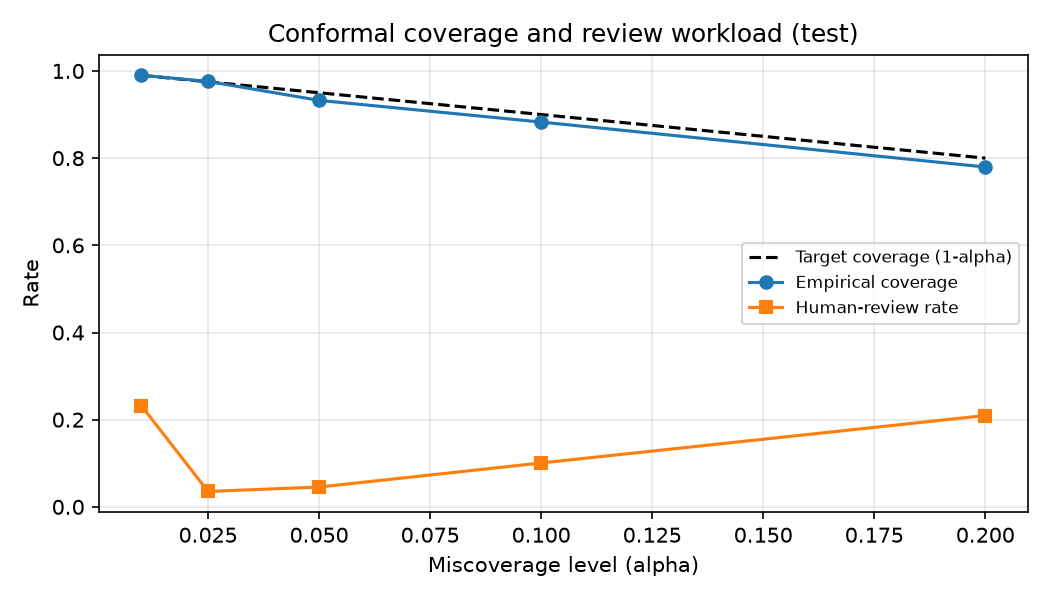
\includegraphics[
    width=\columnwidth,
    keepaspectratio
]{../figures/conformal/coverage_vs_workload.png}
\caption{Empirical conformal coverage and human-review workload across evaluated
miscoverage levels.}
\label{fig:conformal_workload}
\end{figure}
\subsection{Autoencoder Latent-Space Analysis}
A t-SNE analysis was performed on 5,000 held-out transactions using the
32-dimensional DAE bottleneck representation. The resulting class-based
silhouette score was 0.1095.
The visualization in Fig.~\ref{fig:tsne} shows partial structural separation but
substantial overlap between legitimate and fraudulent transactions. The weak but
non-zero separation is consistent with the role of the DAE as an unsupervised
anomaly detector rather than a standalone fraud classifier. The representation
therefore provides complementary structural information rather than a clean
fraud decision boundary.
\begin{figure}[t]
\centering
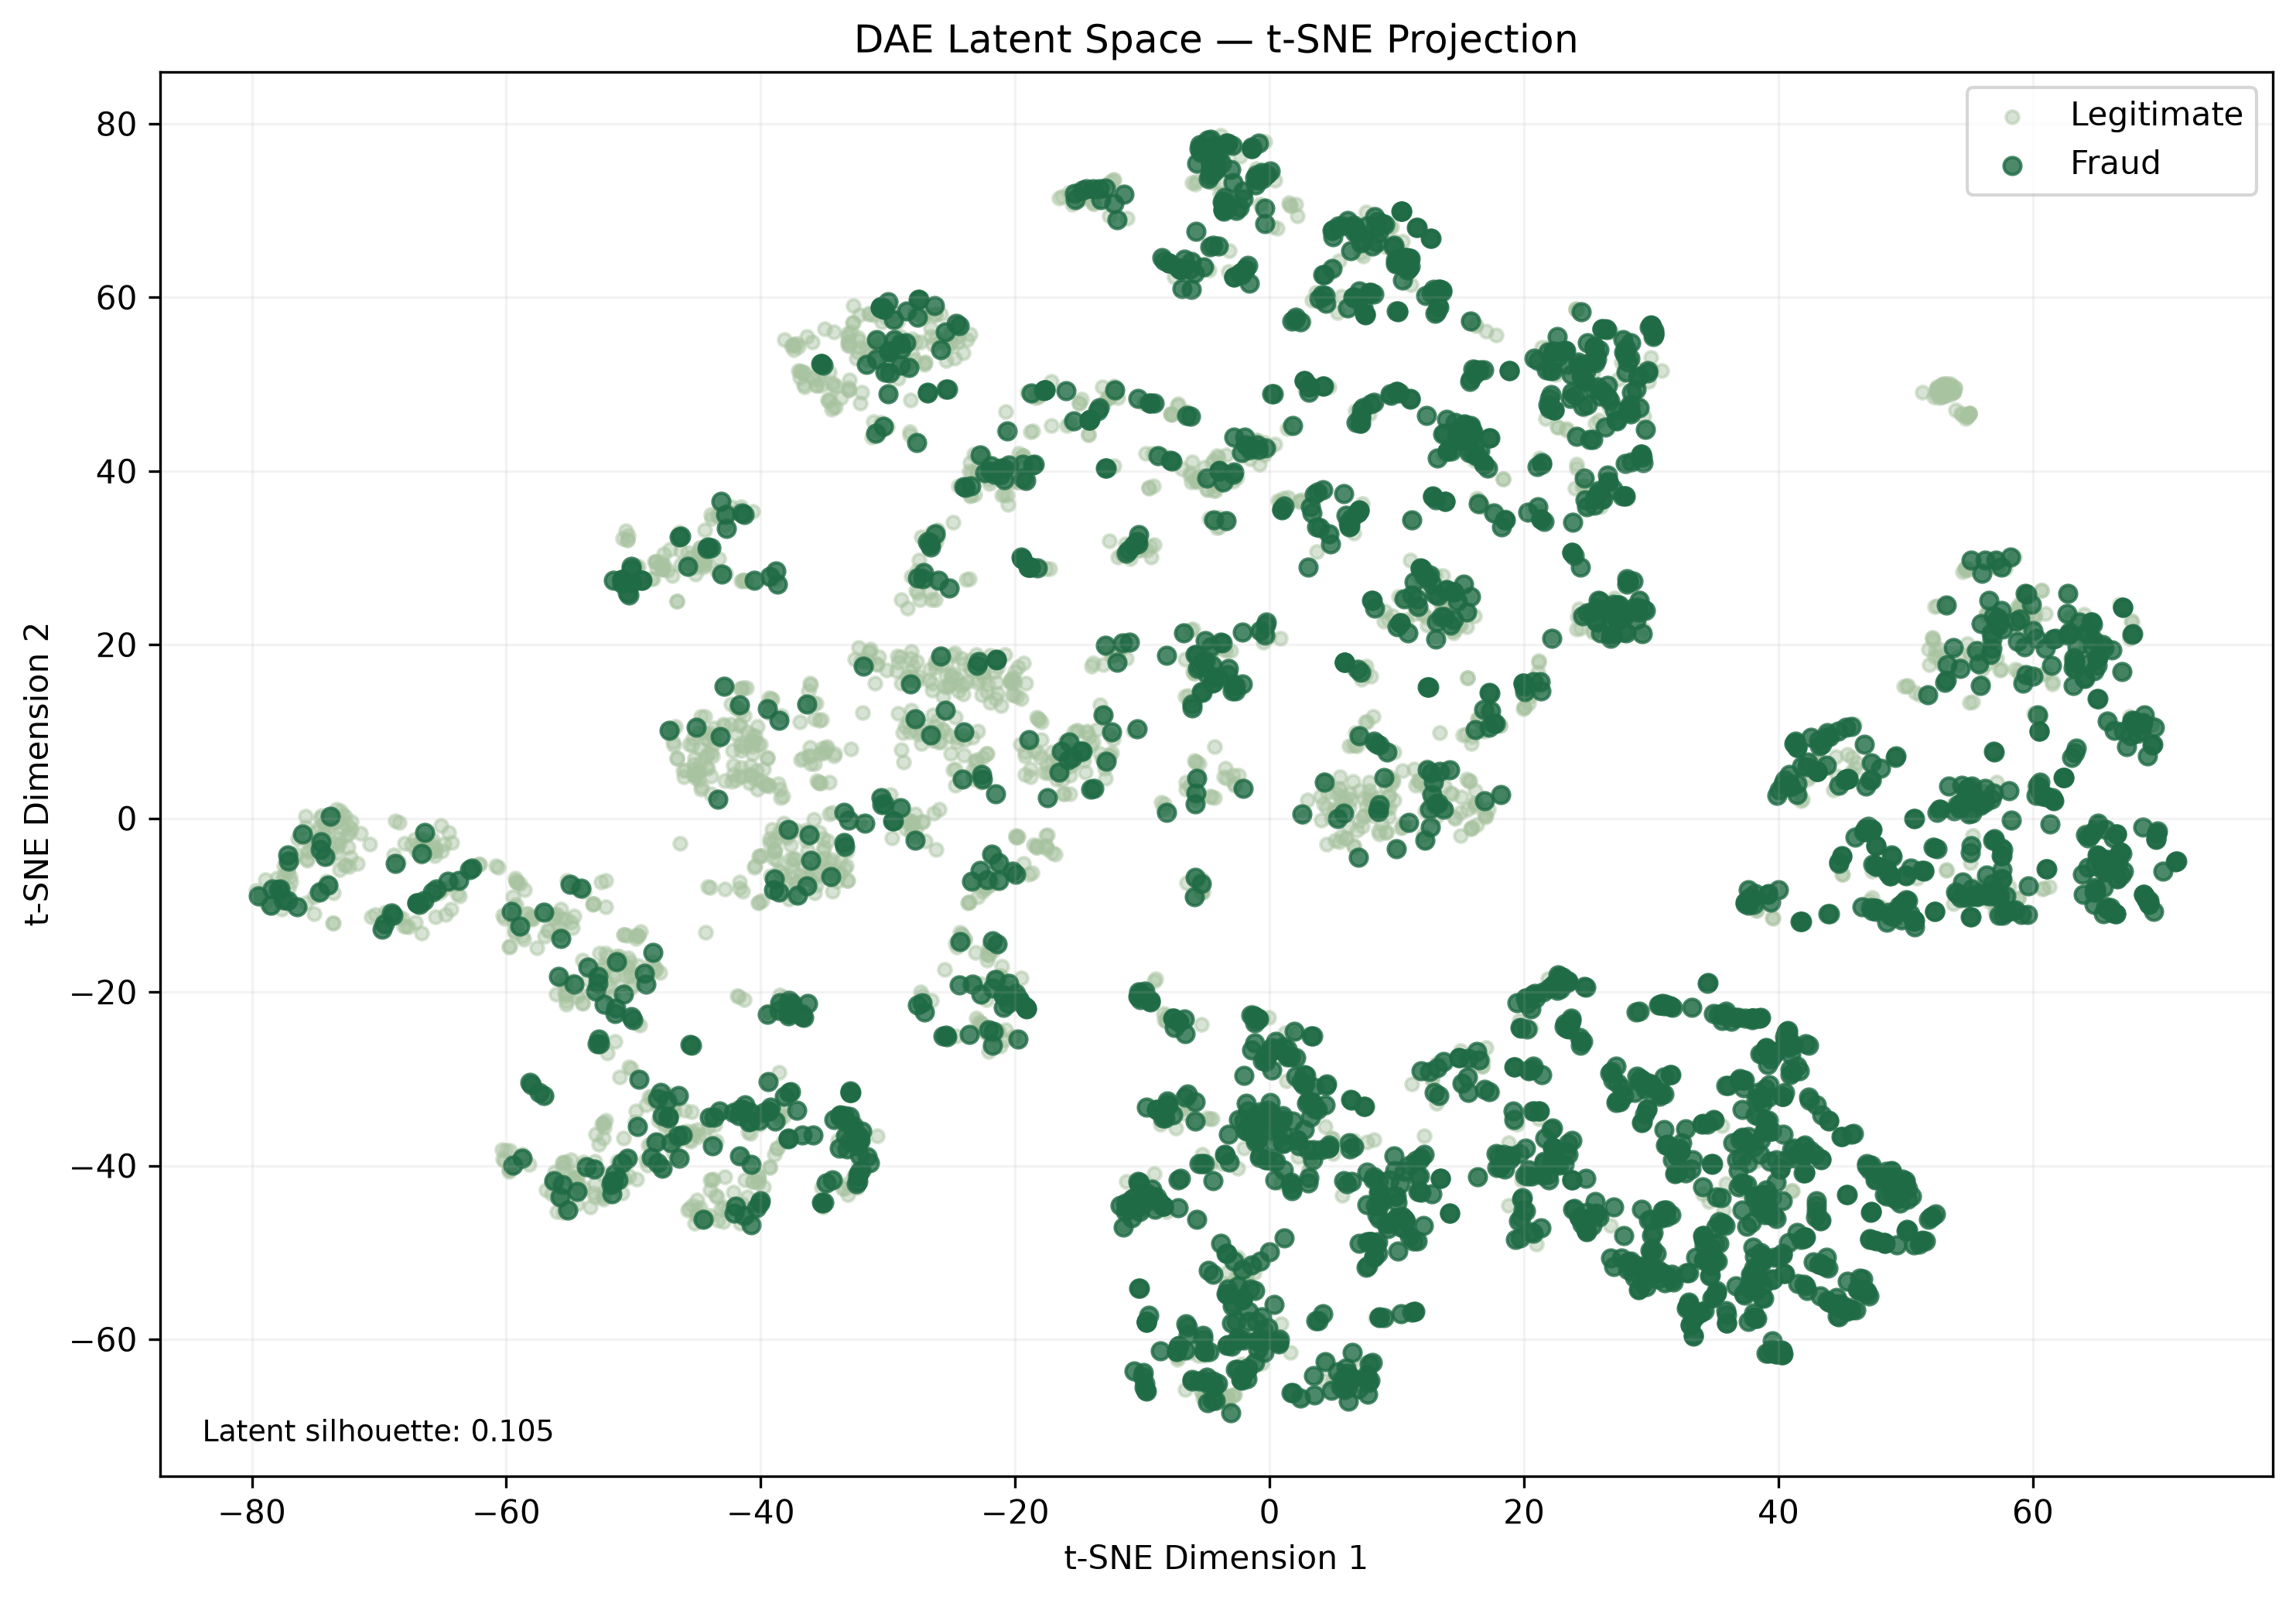
\includegraphics[
    width=\columnwidth,
    height=0.38\textheight,
    keepaspectratio
]{../figures/autoencoder_latent/tsne_latent_space.png}
\caption{t-SNE projection of the 32-dimensional DAE bottleneck representation.}
\label{fig:tsne}
\end{figure}
\subsection{SHAP Analysis}
SHAP analysis was used to inspect the DAE anomaly component. Across independent
global samples, the mean Spearman correlation of feature rankings was 0.8924,
while mean top-feature Jaccard similarity was 0.4762.
Figure~\ref{fig:shap_global} shows the global SHAP importance profile for the DAE
anomaly component. In the sampled analysis, \texttt{addr1} receives the strongest
global anomaly attribution. The high mean Spearman rank correlation indicates
that the broader ordering of feature importance is relatively stable across
independent samples, although the lower mean top-feature Jaccard similarity
shows that membership of the exact top-feature set is less stable.
Importantly, these attributions explain reconstruction anomaly rather than the
final fused fraud probability. The prominence of \texttt{addr1} therefore should
not be interpreted as evidence that it is the strongest predictor of fraud.
\begin{figure}[t]
\centering
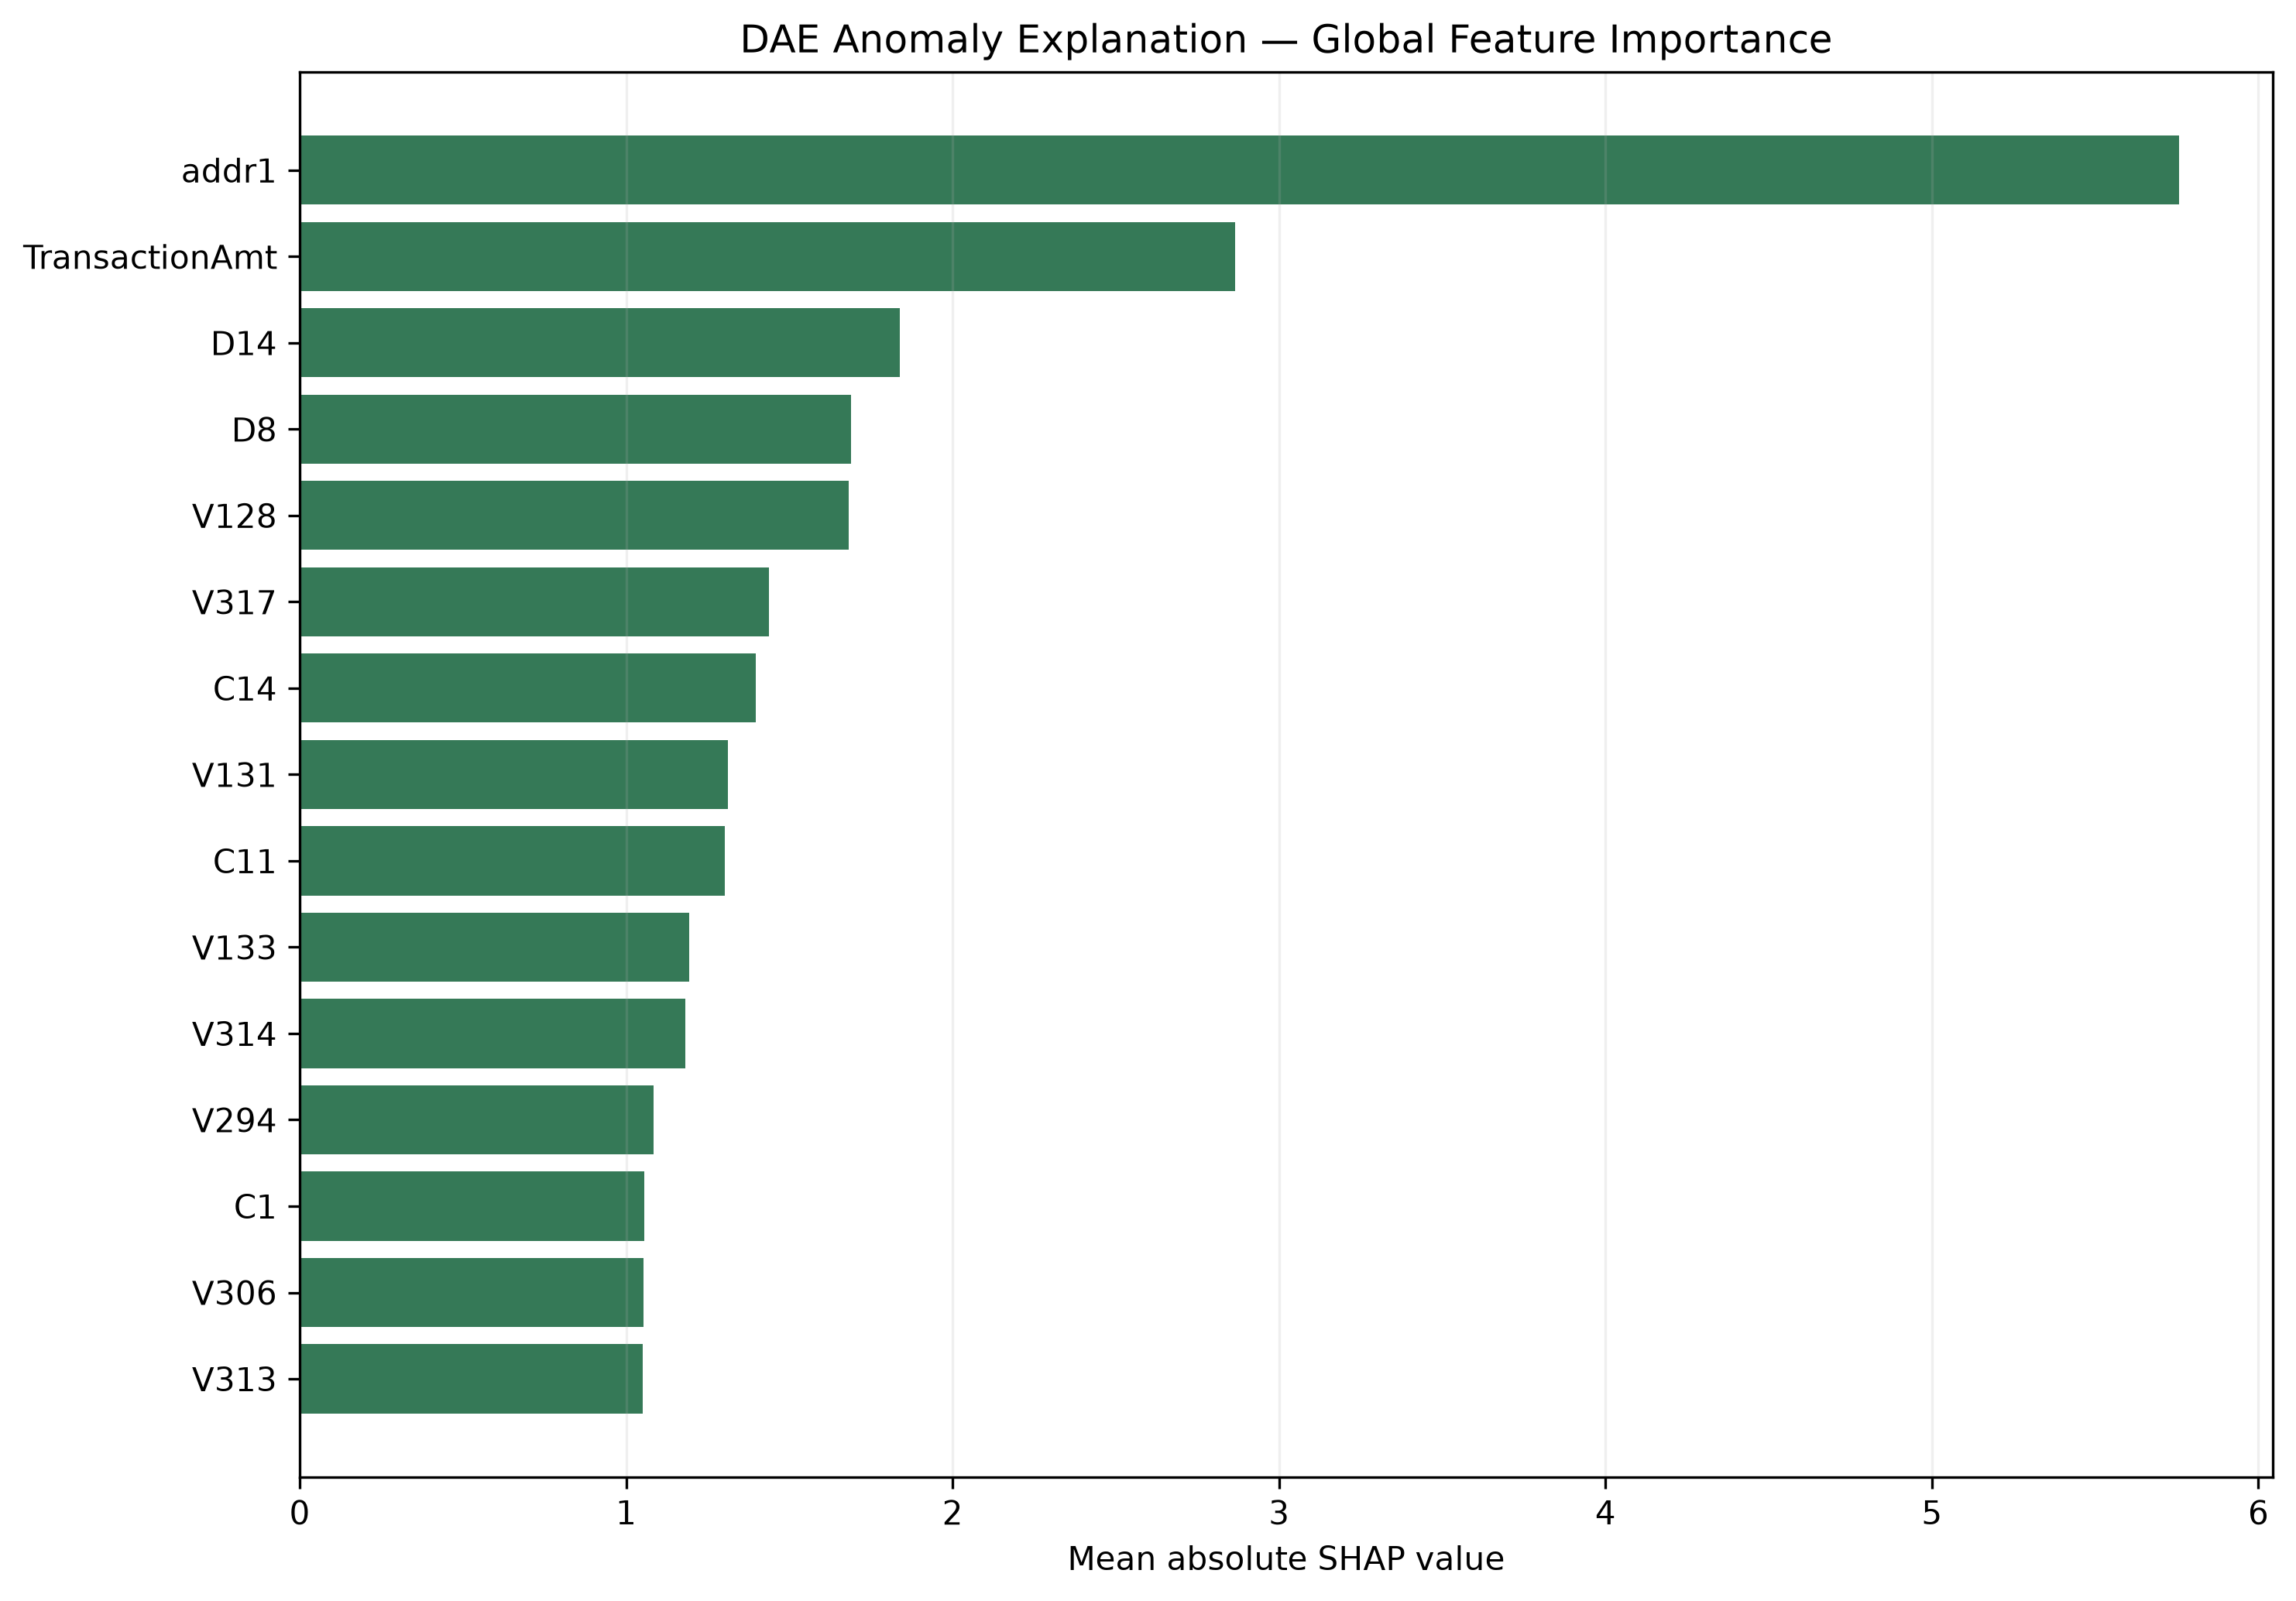
\includegraphics[
    width=\columnwidth,
    keepaspectratio
]{../figures/explainability/dae_shap_global_importance.png}
\caption{Global SHAP feature importance for the DAE reconstruction-anomaly
component.}
\label{fig:shap_global}
\end{figure}
\subsection{CPU Inference Performance}
The neural inference path was benchmarked on CPU using 10 warm-up iterations and
50 measured iterations per batch size. The benchmark includes the DAE, FT-CAT,
transaction-history feature assembly, and learned gate. It excludes HTTP/Pydantic
overhead, disk I/O, SHAP computation, and conformal decision logic.
\begin{table}[t]
\caption{End-to-end neural CPU inference benchmark.}
\label{tab:latency}
\centering
\begin{tabular}{@{}rrrr@{}}
\toprule
Batch & Median (ms) & P99 (ms) & Throughput \\
\midrule
1   & 6.56   & 26.95  & 128 tx/s \\
32  & 14.90  & 24.08  & 2,092 tx/s \\
128 & 44.94  & 67.56  & 2,746 tx/s \\
512 & 189.73 & 290.84 & 2,693 tx/s \\
\bottomrule
\end{tabular}
\end{table}
Batch size 128 produced the highest tested throughput at approximately 2,746
transactions per second. At batch size 1, median neural inference latency was
6.56 ms. Component-level profiling showed that FT-CAT dominates the neural
compute path, whereas learned-gate inference itself is lightweight.
Figure~\ref{fig:throughput} shows that throughput increases substantially with
batching before reaching its highest tested value at batch size 128. Throughput
rises from approximately 128 transactions per second at batch size 1 to 2,746
transactions per second at batch size 128, before remaining approximately flat
at 2,693 transactions per second for batch size 512. Moderate batching therefore
provides substantial computational efficiency, while increasing the batch size
beyond 128 produced no additional throughput benefit in the tested CPU
environment.
These measurements describe model-side neural inference and should not be
interpreted as complete HTTP API latency.
\begin{figure}[t]
\centering
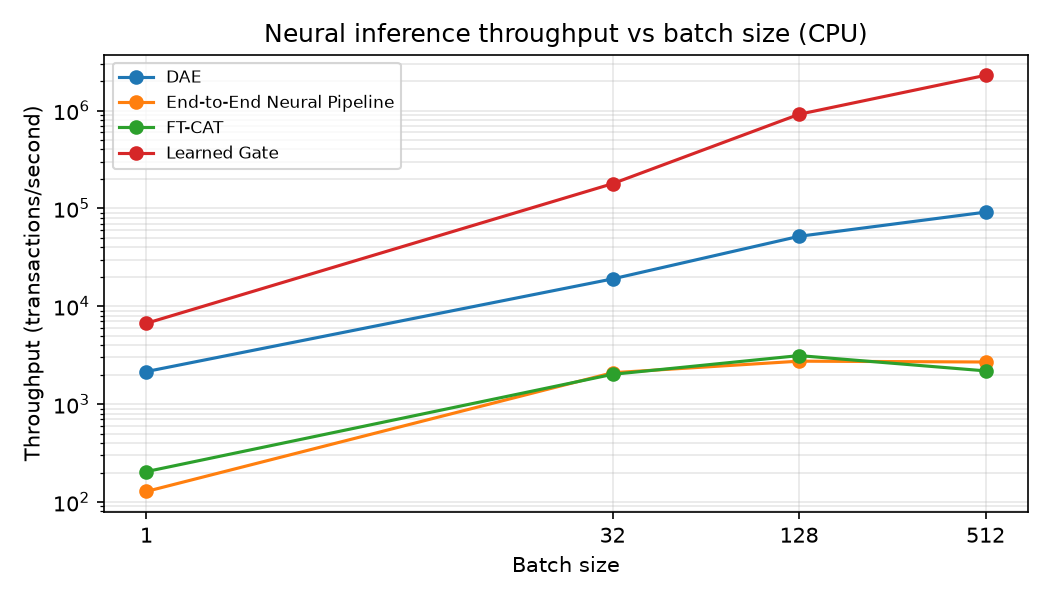
\includegraphics[
    width=\columnwidth,
    keepaspectratio
]{../figures/inference_benchmark/inference_throughput.png}
\caption{Measured neural inference throughput across evaluated batch sizes on CPU.}
\label{fig:throughput}
\end{figure}
\subsection{Deployment and Serialization}
The trained DAE, FT-CAT, and learned gate were successfully serialized to both
PyTorch EXIR and ONNX representations. Export-time parity checks compare
serialized outputs with their PyTorch reference implementations.
The product additionally exposes a FastAPI scoring interface and a Streamlit
analyst dashboard. The dashboard surfaces prediction, batch analysis, model
insights, conformal triage, explainability, and artifact-readiness information.
\section{Discussion and Limitations}
\label{sec:discussion}
The experiments demonstrate the value of treating fraud detection as a triage
problem rather than forcing every transaction into an automatic binary decision.
The supervised FT-CAT branch provides discriminative fraud evidence, while the
DAE contributes a complementary anomaly signal. Learned gating provides a
flexible mechanism for combining these signals with transaction history.
The conformal results expose an important operational trade-off. The system
achieves 98.99\% empirical marginal coverage on the chronological test set at
the 99\% target, but approximately 23.19\% of transactions require human review.
At this conservative operating point, no test transactions are automatically
blocked. Therefore, the current configuration is better characterized as a
high-coverage approval-and-review system than as a fully automated
fraud-blocking system.
A second limitation is class-conditional behavior. Marginal coverage is close
to the nominal target, but fraud-class coverage is substantially lower than
legitimate-class coverage. Marginal split conformal prediction does not
guarantee equal class-conditional coverage.
A third limitation concerns the assumptions behind conformal prediction.
Finite-sample marginal coverage applies under exchangeability between
calibration and future examples. Financial transaction data are chronological
and may undergo temporal or adversarial distribution shift. Consequently,
98.99\% should be reported as observed chronological test coverage, not as an
unconditional guarantee for future production traffic.
The SHAP implementation is also intentionally scoped. Current explanations
describe the DAE anomaly component and do not provide a complete attribution of
the final learned-gate decision. Extending explainability to the complete fused
system is an important direction for future work.
The fixed-coefficient and learned-gating comparison also requires careful
interpretation. The learned gate incorporates transaction-history activity and
amount-intensity features in addition to the DAE and FT-CAT signals, whereas a
simple fixed-weight fusion uses only the two model scores. Improvements from the
learned system therefore cannot be attributed exclusively to nonlinear fusion;
the additional causal history context is also part of the learned-gate design.
Finally, the latency benchmark measures the neural computation path rather than
complete request-to-response service latency. Production deployment would
require additional benchmarking of network overhead, request validation,
concurrency, monitoring, and data retrieval.
\section{Conclusion}
\label{sec:conclusion}
We presented an end-to-end financial fraud detection and uncertainty-triage
engine combining an FT-CAT Transformer, a denoising autoencoder, learned hybrid
gating, and split conformal prediction.
The system achieved 98.99\% empirical marginal coverage at a nominal 99\% target
on the chronological held-out test set while routing 23.19\% of transactions to
human review. The results demonstrate the practical role of uncertainty-aware
triage: rather than forcing every prediction into an automated action, the
system explicitly identifies cases requiring analyst intervention.
The deployment prototype supports FastAPI serving, an analyst-facing Streamlit
dashboard, SHAP-based anomaly explanations, and EXIR and ONNX serialization.
CPU benchmarking demonstrated a median batch-1 neural inference latency of
6.56 ms and peak tested throughput of approximately 2,746 transactions per
second.
Future work should investigate class-conditional conformal calibration,
distribution-shift monitoring, fused-model explanations, and alternative
operating points that support safe automatic blocking.
\section*{Tools and Acknowledgements}
We used AI-assisted tools, including ChatGPT, to support code debugging,
software review, test development, and wording refinement during the project.
All experiments, reported metrics, implementation decisions, and final
materials were reviewed and validated by the authors.
We acknowledge the AI Academy and National Artificial Intelligence Center for
the Deep Learning Cohort I course environment and project framework. We also
acknowledge Vesta Corporation and the IEEE Computational Intelligence Society
for the IEEE-CIS Fraud Detection dataset~\cite{ieeecis2019} used to train and
evaluate the system.
\begin{thebibliography}{9}
\bibitem{vaswani2017attention}
A. Vaswani et al.,
``Attention is all you need,''
in \emph{Proc. Advances in Neural Information Processing Systems}, 2017.
\bibitem{gorishniy2021revisiting}
Y. Gorishniy, I. Rubachev, V. Khrulkov, and A. Babenko,
``Revisiting deep learning models for tabular data,''
in \emph{Proc. Advances in Neural Information Processing Systems}, 2021.
\bibitem{lundberg2017unified}
S. M. Lundberg and S.-I. Lee,
``A unified approach to interpreting model predictions,''
in \emph{Proc. Advances in Neural Information Processing Systems}, 2017.
\bibitem{vovk2005algorithmic}
V. Vovk, A. Gammerman, and G. Shafer,
\emph{Algorithmic Learning in a Random World}.
New York, NY, USA: Springer, 2005.
\bibitem{angelopoulos2023gentle}
A. N. Angelopoulos and S. Bates,
``Conformal prediction: A gentle introduction,''
\emph{Foundations and Trends in Machine Learning},
vol. 16, no. 4, pp. 494--591, 2023.
\bibitem{ieeecis2019}
IEEE Computational Intelligence Society and Vesta Corporation,
``IEEE-CIS Fraud Detection,''
Kaggle competition, 2019. [Online]. Available:
\url{https://www.kaggle.com/competitions/ieee-fraud-detection}
\end{thebibliography}
\end{document}
